\documentclass{article}

\author{Wenyu Jing, Shivam Duhan, Chengming Zhang, Mingqi Li}
\title{\textbf{DRL Enabled AI Factorio Player}}

\usepackage{natbib}
\usepackage{graphicx}

\begin{document}

\maketitle

\section{Introduction}
We are creating a reinforcement learning agent to play the optimization game Factorio, a game in which you build and maintain factories. The agent will be mining resources, researching technologies, building infrastructure, automating production and fighting enemies. 
\begin{center}
  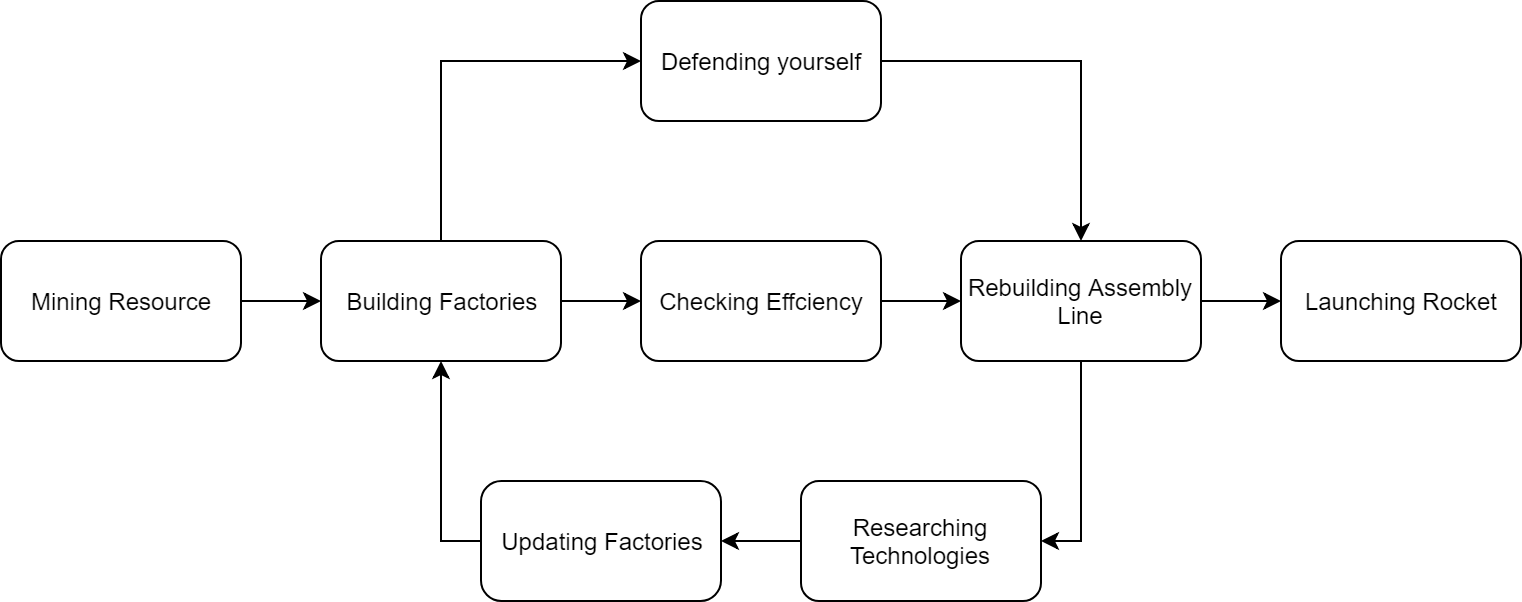
\includegraphics[width=11cm, height=4cm]{47900.png}}
\end{center}

\section{Why Factorio} 
Factory optimization is typically carried out using Linear programming. Neural Networks can probably do a better job but require a lot of data which is not feasible in current factories. Using Reinforcement learning to train an agent to manage a factory simulation and then transferring that learning to the real world is our best bet to dramatically increase efficiency and productivity and enable everyone in the world to afford high quality manufactured goods. Factorio provides us with the perfect environment to create such an agent. It includes all the activities typically associated with the CEO of a company and more, with immediate reward signals that can be optimized. It allows for extensive modification using the in-game debugging mode and the Lua programming language which will allow us to insert our agent and interface it with the game effortlessly. The challenge is that it is an incredibly complex games, at least an order of magnitude more difficult than games (eg. Atari games ) typically targeted by reinforcement learning agents. A reinforcement learning agent who can play Factorio well can make factories, run companies, and design supply chains much better than humans and will help us make everything cheaper. The agent can also control Energy production. 

\section{Optimization scope}


There are 5 main things that can be optimized using our reinforcement learning agent: 
\begin{itemize}
    \item resource acquisition,
    \item technology research,
    \item infrastructure projects,
    \item production automation, and
    \item military might
\end{itemize}
To keep the agent manageable, we will not focus on the military aspects by making a custom mod with no enemies. We will also not focus on doing research to build rockets. All of our efforts will be focused on maximizing production and logistical efficiency.


\section{Factorio Gameplay Experience}
One of our team members, Chengming Zhang, has played Factorio for 62 hours. He found the game to be very difficult because of the amount of freedom that the game offers. To achieve the final goal of the game which is to build a rocket ship, one must keep the factory production line efficient yet productive. Chengming had to spend a good amount of time on the official game wiki page to learn critical information like how to boost production efficiency, make a particular part, etc. To run an efficient factory, one of the most important things is to have the machines arranged so that all machines can run non-stop, meaning the throughput and latency are perfect. A healthy production rate is key.

\section{Work Load Assignment}
There are 4 main parts of the project, the yellow marking blocks will be programmed using python, and the purple marked block will be programmed using lua. 

\begin{center}
  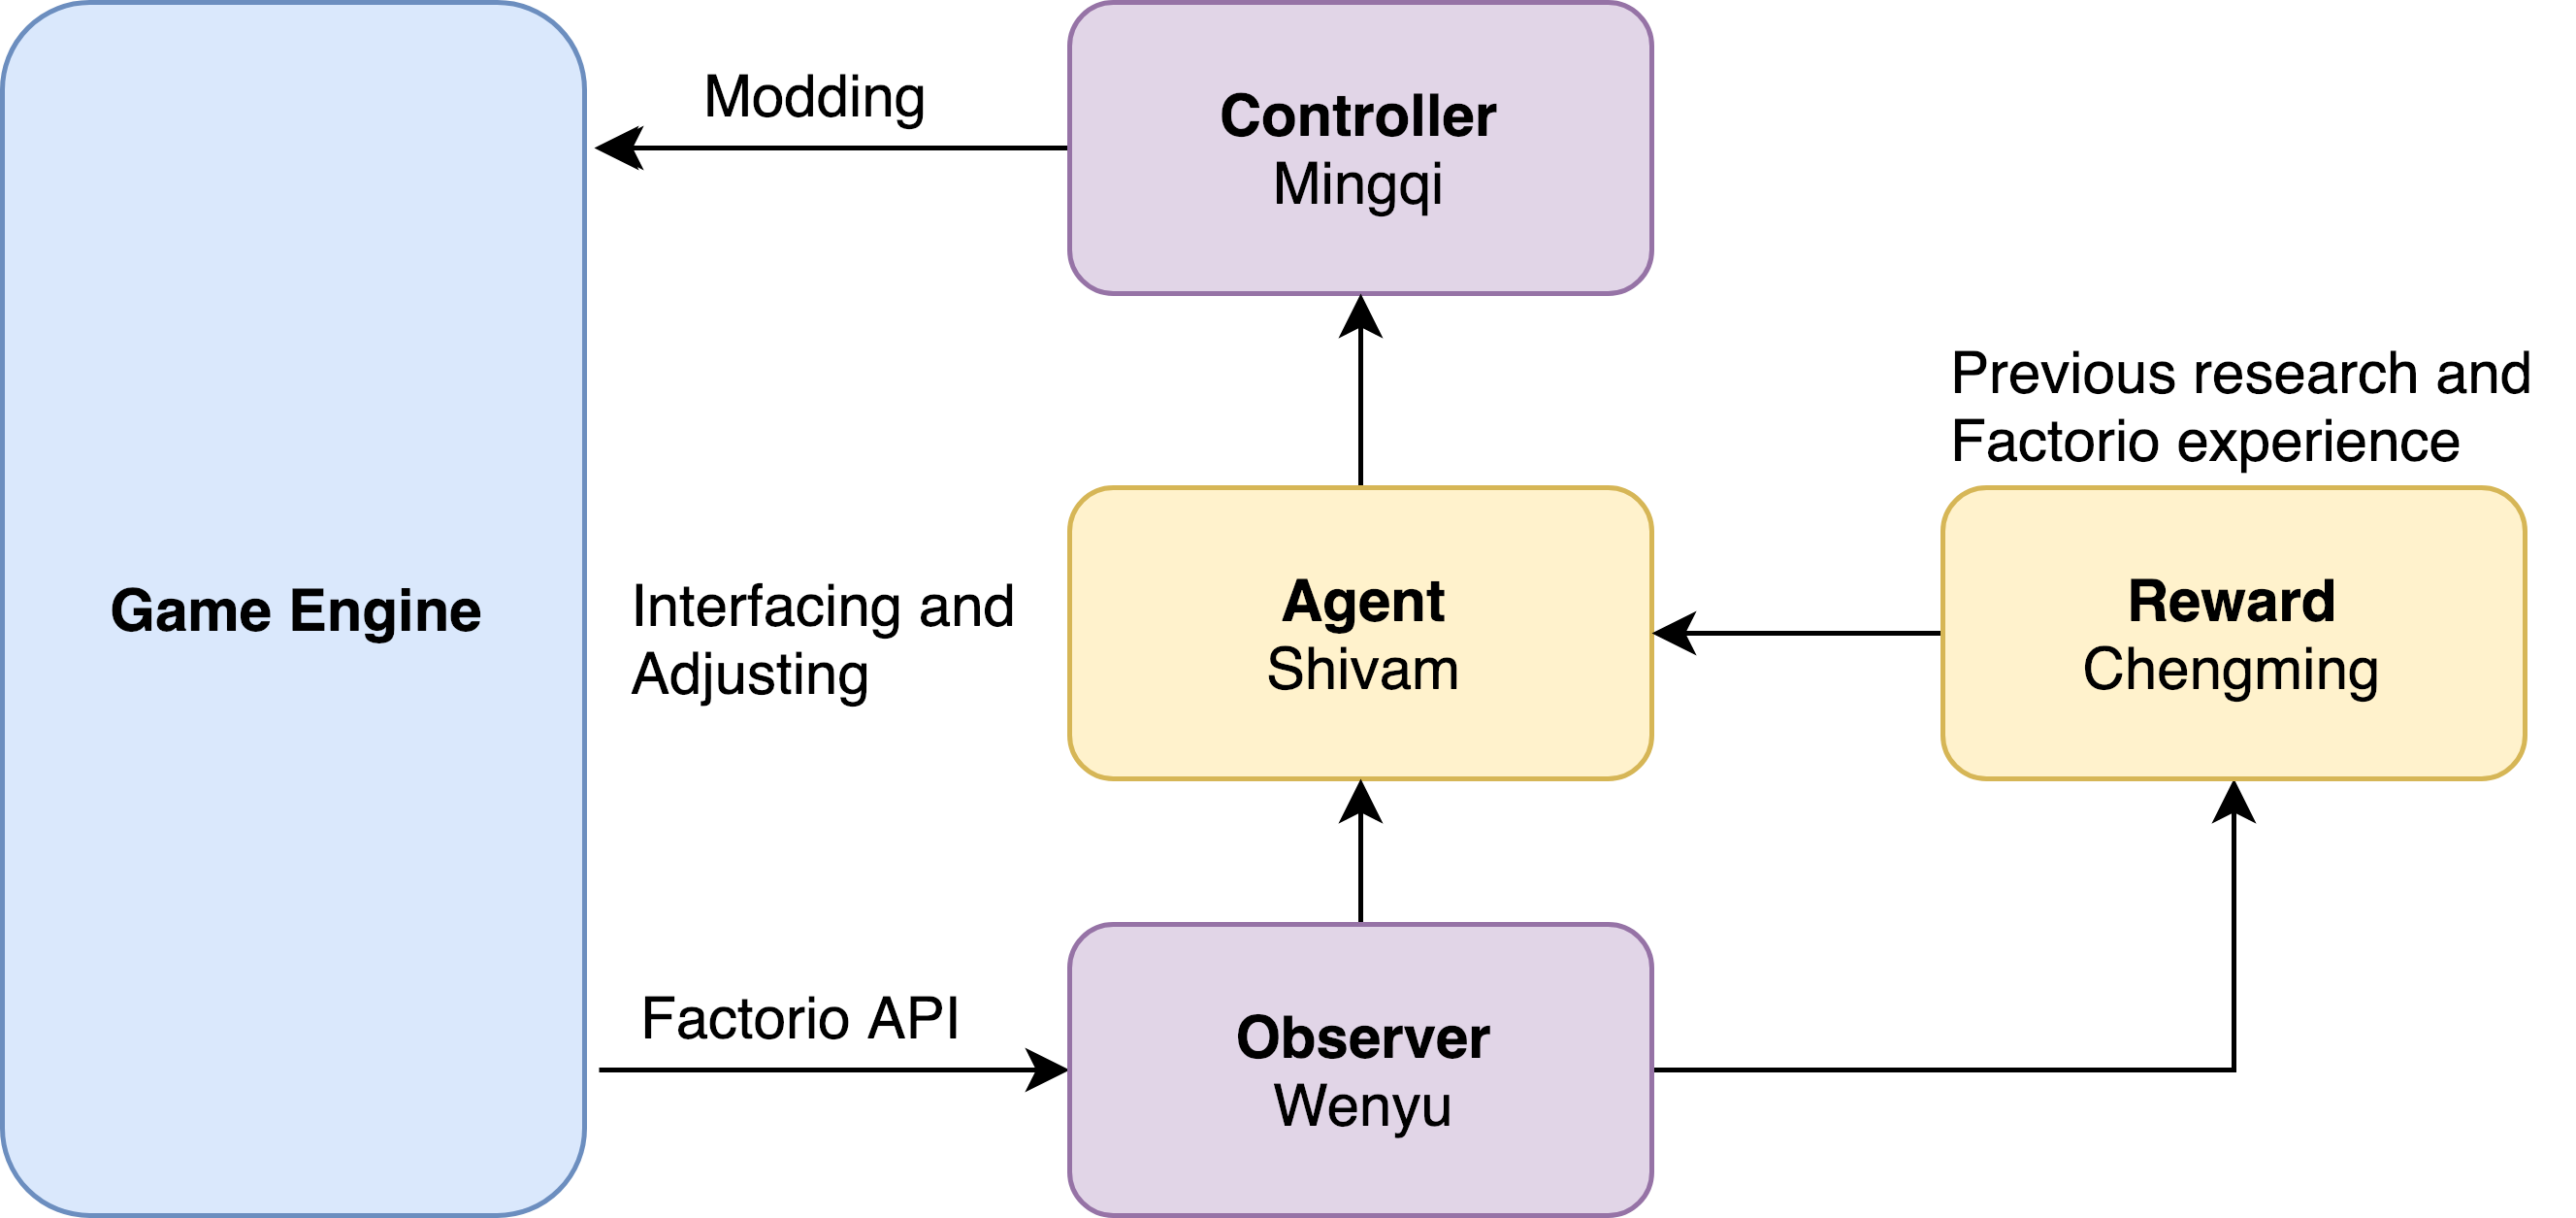
\includegraphics[width=11cm, height=5cm]{download.png}
\end{center}

\begin{itemize}
    \item  Controller - In charge of the game via modding capability. The controller follows the commands issued by the agent. - Mingqi
    \item  Agent - Takes input from the observer, outputs to the controller, and adjusts behavior according to the  reward.- Shivam
    \item  Observer - Reads key metrics from the game engine using the Factorio API, written in Lua. - Wenyu
    \item  Reward - Specifies key metrics and how to optimize them, sets limits on the agent’s scope. - Chengming
    
\end{itemize}
   
    
\section{Project Milestones}

\begin{itemize}
   \item Week 5: Submit Project Proposal and collect data for human game play for latter comparison and also to gain a better understanding of the game.
   \item Week 6: Come up with Controller, Agent, Observer, and Reward design framework. Do small scale testing in the game. Define reward function. Define small scale testing to limit the game play initially for testing. Define success. Create virtual machine on server to run training program.
   \item Week 7: Submit Midterm Evaluation and peer evaluation forms. Re-think current strategy. 
   \item Week 8: Training and Evaluation model for \textbf{Navigation in game}
   \item Week 9: Training and Evaluation model for \textbf{Finding resources}
   \item Week 10: Training and Evaluation model for \textbf{Mining resource}
   \item Week 11: Second Midterm Evaluation. Re-think current strategic. 
   \item Week 12: Training and Evaluation model for \textbf{Autonomous Crafting and picking resource}
   \item Week 13: Training and Evaluation model for be able to manufacture \textbf{item "circuit I"}
   \item Week 14: Training and Evaluation model for be able to manufacture \textbf{item "circuit II"}
   \item Week 15: Training and Evaluation model for be able to manufacture \textbf{item "circuit III"}
   \item Week 16: Submit finial report, present result in class, and present in conference.
    
\end{itemize}

\section{Definition of success}
An agent will able to create a \textbf{self-sustaining} factory. 
\bibliographystyle{plain}
\begin{thebibliography}{9}

\bibitem{1} 
Lua For Programmers Part 1: Language Essentials,
\\\texttt{http://ebens.me/post/lua-for-programmers-part-1/}

\bibitem{2} 
Programming in Lua (first edition),
\\\texttt{http://www.lua.org/pil/contents.html}

\bibitem{3} 
Learn X in Y Minutes Where X=lua,
\\\texttt{https://learnxinyminutes.com/docs/lua/}

\bibitem{4} 
Lua Documentation,
\\\texttt{https://www.lua.org/docs.html}

\bibitem{5} 
Factorio Modding,
\\\texttt{https://wiki.factorio.com/index.php?title=Modding}

\bibitem{6} 
Factorio API,
\\\texttt{https://lua-api.factorio.com/latest/}

\end{thebibliography}
\end{document}
